\documentclass[conference, 10pt]{IEEEtran}
\IEEEoverridecommandlockouts
% The preceding line is only needed to identify funding in the first footnote. If that is unneeded, please comment it out.
\usepackage{cite}
\usepackage{amsmath,amssymb,amsfonts}
\usepackage{algorithmic}
\usepackage{graphicx}
\usepackage{textcomp}
\usepackage{xcolor}
\def\BibTeX{{\rm B\kern-.05em{\sc i\kern-.025em b}\kern-.08em
    T\kern-.1667em\lower.7ex\hbox{E}\kern-.125emX}}
\graphicspath{"."}


\begin{document}

\title{ML Reconstruction of 3D Neurovascular Models from Biplane Views\\
}

\author{\IEEEauthorblockN{Connor Chin}
\IEEEauthorblockA{\textit{B.S student of Computer Science} \\
\textit{UCLA}\\
Los Angeles, USA \\ 
connorchin@g.ucla.edu}
\and
\IEEEauthorblockN{Kevin Li}
\IEEEauthorblockA{\textit{B.S student of Computer Science} \\
\textit{UCLA} \\
Los Angeles, USA \\
kevinli120@yahoo.com}
}

\maketitle

\begin{abstract}
    This paper is a report of 3D neurovascular models from multiple biplane views. 
    It introduces a deep learning approach to the model and various methods implemented in an attempt to reconstruct these models. 
    We also discuss issues encountered, performance, and possible fixes. 
    There have been other machine learning approaches to this problem, but none use deep learning.
    Our hope was that deep learning would provide a versatile, complex way of reconstructing the vascular structure in the brain.
    The discussion and conclusion, however, will show that the methods we attempted did not yield satisfiable results. 
    We will provide an analysis on our architecture and possible design flaws that hindered the network performance.
\end{abstract}

\begin{IEEEkeywords}
reconstruction, machine learning, deep learning, vascular structure, morphology
\end{IEEEkeywords}

\section{Preprocessing}
We start with 61 morphology files provided by the BraVa dataset (http://cng.gmu.edu/brava). Each file contains extracted morphological measurements of 61 adult subjects. From these measurements, we obtain a 3D construction of the vascular structure of each patient's brain. The model allows us to take six images representing different views of the brain's vascular structure. These images can be seen in figure 1.

\begin{figure}[h]
    \centering
    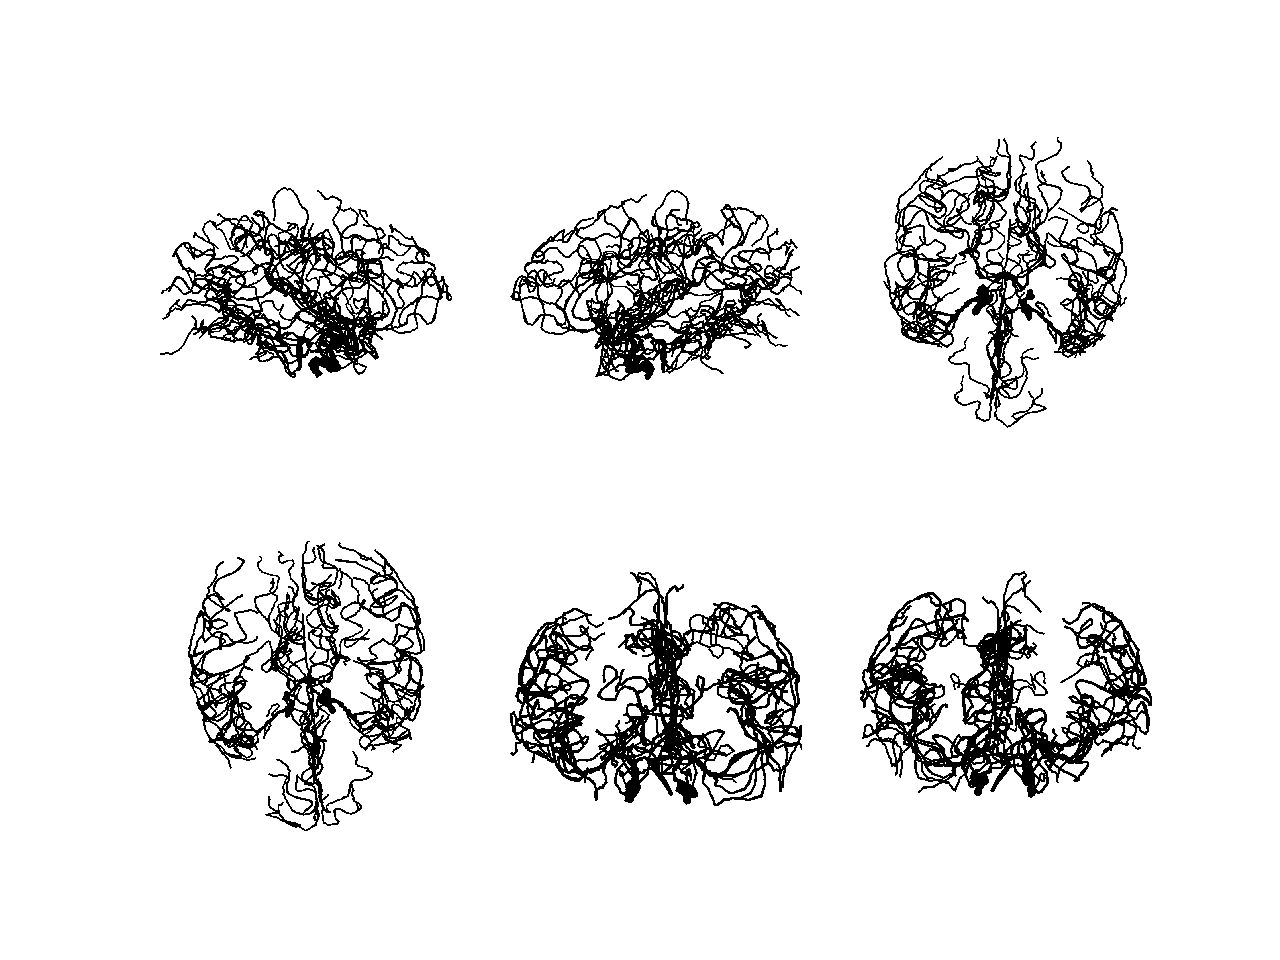
\includegraphics[scale=0.21]{figure_1.png}
    \caption{Six Biplane Views}
\end{figure}

These biplane views will be our input for the neural network and were resized to single-channel 256x256 images to simplify and reduce the number of features. Furthermore, we found that any lower resolution resulted in inaccurate input images, namely disconnected branches of some blood vessels in the structure. The 3D models obtained from the morphology file are now converted to a voxelized representation. This makes the ground truth 3D models viable for this application. Each 3D ground truth model was set to a size fo 64x64x64. Similar to our evaluation of the biplane input images, this number of voxels was the minimum required to have an accurate ground truth representation.

\begin{figure}[h]
    \centering
    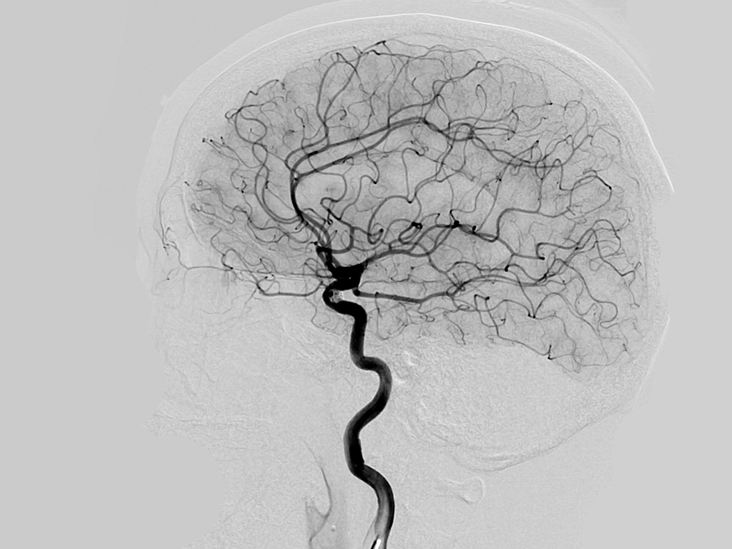
\includegraphics[scale=0.25]{figure_2.jpg}
    \caption{X-Ray Angiography}
\end{figure}

To further simplify the input to our neural network, instead of concatenating six consecutive single-channel biplane images for our input, we instead chose to combine these images into a single, six-channel image. Then, the convolution levels in our network would be less computational expensive and it working with an easier input.

We may justify the practicallity of these biplane input images by evaluating the method by which doctors obtain them in practice. X-ray angiography helps highlight blood vessels in the brain as seen in figure 2. With this biplane view, current deep learning methods \cite{Angiography Segmentation} can be applied to this image as a way to extract the blood vessels into another image similar to our input data for this project. In practice, doctors attempting to diagnose neurovascular diseases may now use X-ray angiography to obtain biplane views of the cerebrovascular structure. Hopefully with the proposed model, they may now reconstruct the vessel structure from these images.

Although directly reconstructing 3D models from 2D images seems to be an intuitive method, we also considered--instead of converting 2D images into 3D reconstructions--generating morphological data from these biplane views to later be converted into 3D reconstructions of the cerebrovascular structure. There are already frameworks in place for converting these neuromorphology files into 3D models, so this method did not seem too far-fetched. However, we found that directly converting the images would be more practical because a direct reconstruction model would be more helpful and eliminate the need for more third-party applications in generating the 3D reconstruction from an X-ray angiography screening.




\section{Methods}
In this section, we discuss our models tested for 3D vascular reconstruction. The current state-of-the-art deep learning 3D- reconstruction models include variants of MVS \cite{MVS}, 3D-R2N2 \cite{3DLSTM}, and 3D VAE/GAN \cite{VAE/GAN} models. In our first review, we noted that although 3D-R2N2 and voxelized MVS models generally achieved better performance on general reconstruction tasks, they generally worked on low resolution output (32x32x32 at most). Due to the complexity of the cerebrovascular network, a high resolution output is required. The VAE/GAN models trade off small differences in performance for a large decrease in training time and difficulty of hyperparameter tuning, and was our natural first choice.

\subsection{3D Autoencoder}
Our first model is a simple implementation of a convolutional/deconvolutional autoencoder. This model primarily serves as pre-training, and the objective is to experiment with dimensionality reduction on our dataset to determine the number of latent dimensions needed for any latent-code-based models. We take the 3D voxelized network as an input and attempt to retrieve it in the output. We used two different types of autoencoders for this experiment: a shallow variant with one fully connected hidden layer and a deep variant with three fully connected hidden layers. 

\subsection{3D Variational Autoencoder}
To improve the autoencoder’s ability to recognize important information, we use a modified generative 3D variational autoencoder for our reconstruction model. A VAE assumes that there is a probabilistic distribution to the input, and tries to infer the parameters of the distribution. This makes it harder to train than a regular autoencoder. Our input to this model is the 256x256 images and the output is the 64x64x64 voxelized reconstruction. This is not identical to a standard VAE in that our goal is to construct a singular output image given a specific input; however, we hypothesize that a VAE suits our task well. This is due to the fact that a projection view may correspond to multiple possible voxel reconstructions, especially at our low resolution. We hope that the VAE can recognize the distribution and likelihood of each reconstruction in it’s latent distribution.

\subsection{3D Generative Adversarial Network}

A generative adversarial network consists of a generator and a discriminator. The generator takes randomly sampled noise as input, and attempts to create voxelized networks that confuse the discriminator. In a traditional GAN, there is no control over the types of images that are generated. As with the VAE, we must modify our network, in this case making it similar to an Information Maximizing GAN (InfoGAN). The InfoGAN adds a latent code input to the generator, which is what we experimented for in the 3D autoencoder. It also adds another network on top of the discriminator, which tries to extract the parameters of the latent distribution. The advantage of GAN networks is that they are generally better at producing discrete visual features where VAEs are likely to blur the output. However, GANs tend to be trickier to train, as shown later.

    
\subsection{Training Details}

\begin{figure}[h]
    \centering
    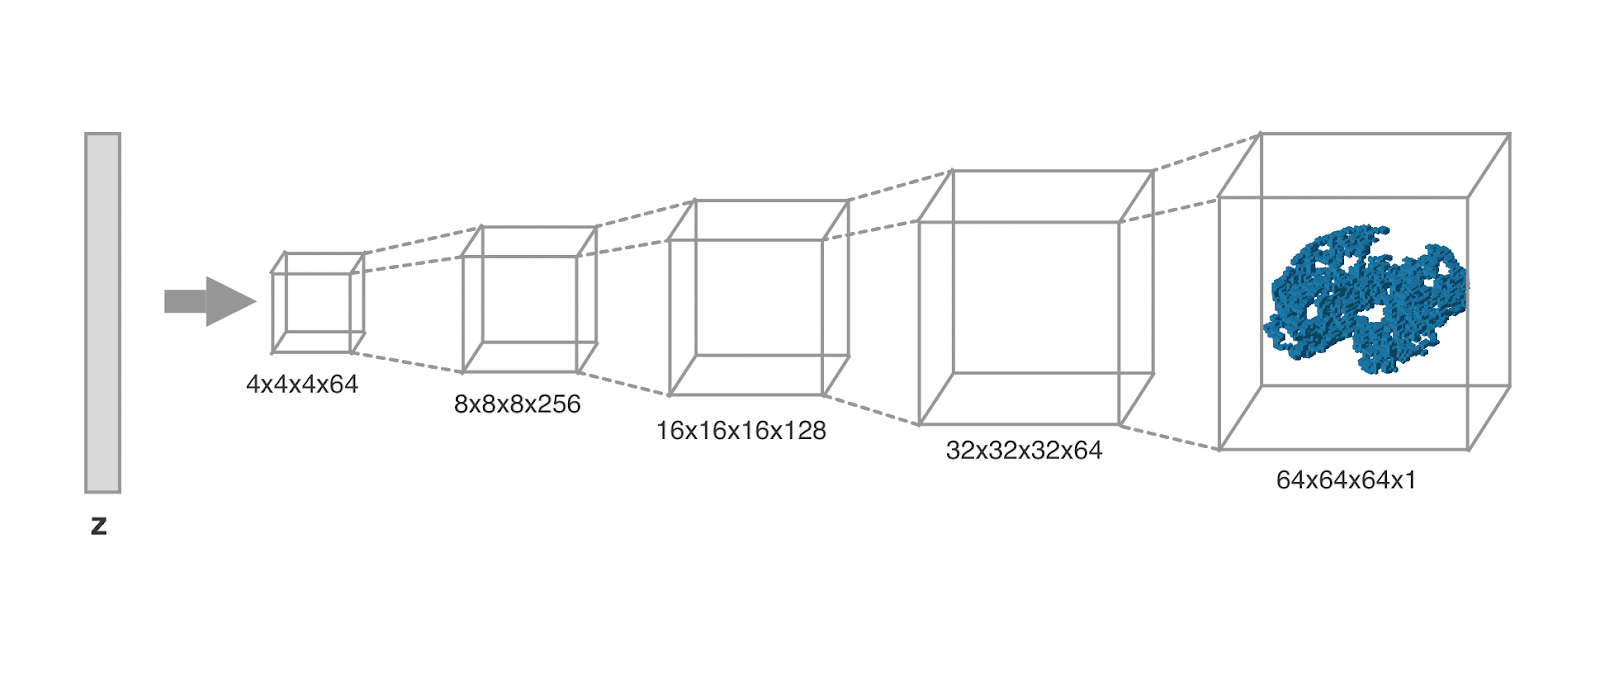
\includegraphics[scale=0.15]{figure_3.png}
    \caption{Generator Network}
\end{figure}

The encoder in each model is implemented as a series of CONV–RELU–POOL–DROPOUT operations, and the decoder is a series of CONVTRANSPOSE–RELU–UPSAMPLE–DROPOUT layers. Dropout is fixed at 0.2 for convolutional layers, and 0.5 for fully connected layers. As shown in Figure 3, each encoder or discriminator consists of four convolutional layers of kernel 3x3x3 and stride 1. For generators the convolution is 3D, and for encoders is 2D. We zero pad the image so that pooling layers can maintain a power of two. The number of filters also increases by a factor of two at every convolutional layer, so that deeper layers have more filters. Instead of standard ReLU layers, we use LeakyReLU layers to minimize dead neurons. The final layer is a fully connected layer to the latent dimension. While typical latent dimensions are around 100, we experimented with a latent dimension of up to 4000. The decoder or generator essentially mirrors the respective encoder/discriminator. As has been standard in the past, we use binary cross-entropy as our loss. After some training, we found that we needed to weigh our loss more heavily toward filled voxels. Thus, our overall loss function is:
\begin{equation}
-(w * y * \log (p) + (1.0 - y) * \log (1.0 - p))
\end{equation}


where w is the weight factor.

For each of these networks, we used ADAM for optimization and a batch size of 4. It should be noted that a larger batch size should increase accuracy. However, the large dimensionality of our output and the number of parameters in our model prohibited any larger batch size.

\section{Discussion}
While training each model, we adjusted the architecture of the network according to the resulting outputs as we saw fit. In several iterations of training the 3D Autoencoder, we found that because the ground truth models were so sparse (approximately 2.65\% of voxels filled in voxel space), our network would converge at a local minimum where it would output all zeros and obtain an accuracy upwards of 95\%.


\begin{figure}[h]
    \centering
    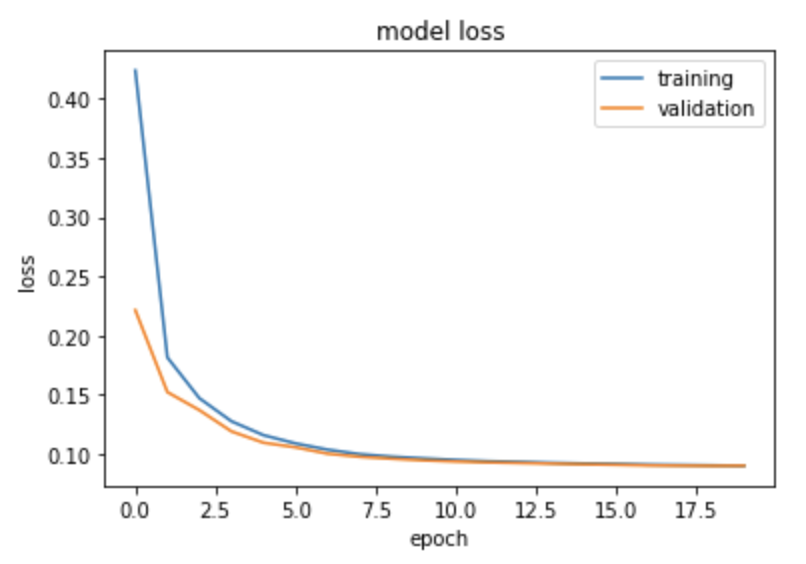
\includegraphics[scale=0.3]{shallow_loss.png}
    \caption{BCE Loss in Shallow Net}
\end{figure}

At first glance, the shallow net with binary cross entropy loss seems to
properly converge at a minimum. However, when viewing the corresponding 3D
model, we see that the model has converged at an empty voxel space.

A potential fix for this problem was to use weighted binary cross entropy loss
to weight the filled voxels more heavily. Though this solution ultimately fixed
this convergence problem, the outputted model was nowhere near accurate. In
fact, we found that the model was too shallow and weighted binary cross entropy 
loss rewarded the network too heavily for filling in voxels. Thus, the
predicted model resembles Fig. 5.

\begin{figure}[h]
    \centering
    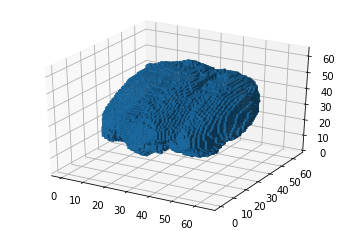
\includegraphics[scale=0.5]{figure_5.png}
    \caption{3D Autoencoder Reconstruction}
\end{figure}

To increase the complexity of our model, we adjusted various hyperparameters 
such as network depth, latent dimension space, and channel depth in an attempt
to discover similarities in the vascular structure. Furthermore, we added
dropout layers to remove some of the neurons that did not contribute to 
the overall model. The increased complexity and novel architecture resulted in
a slightly improved version of the model seen in Fig. 6. 

\begin{figure}[h]
    \centering
    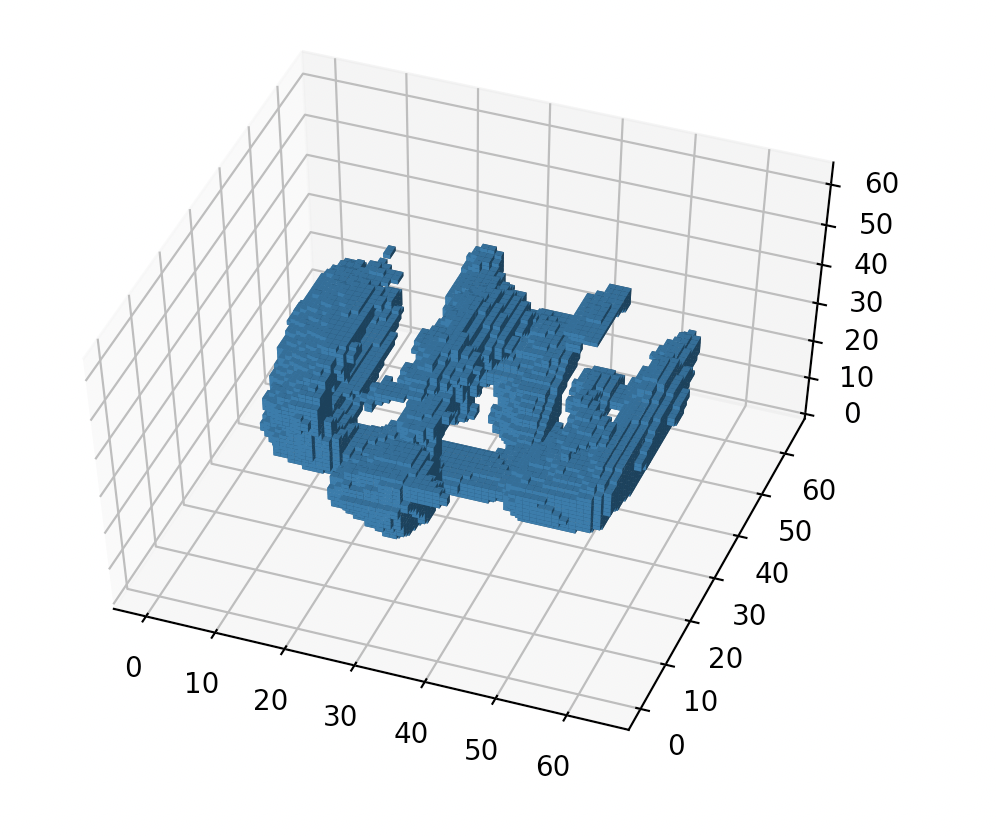
\includegraphics[scale=0.2]{add_dropout.png}
    \caption{Increased Complexity With Weighted BCE Loss}
\end{figure}

As seen in Fig. 6, the network fails to learn any valuable information about 
the vascular structure in general. We also found that the loss in the center of 
the vascular structure was greatest in that region. To compensate, we created a 
custom loss function--based off the weighted binary cross entropy loss--to 
weight those voxels heavily during training. Moreover, we increased the size of 
our network to 46 million parameters to learn complex features in the 
structure. Thus, the increased complexity and custom-weighted loss function 
would, theoretically, help the network learn patterns within the vascular 
structure and produce a complex model. 

\begin{figure}[h]
    \centering
    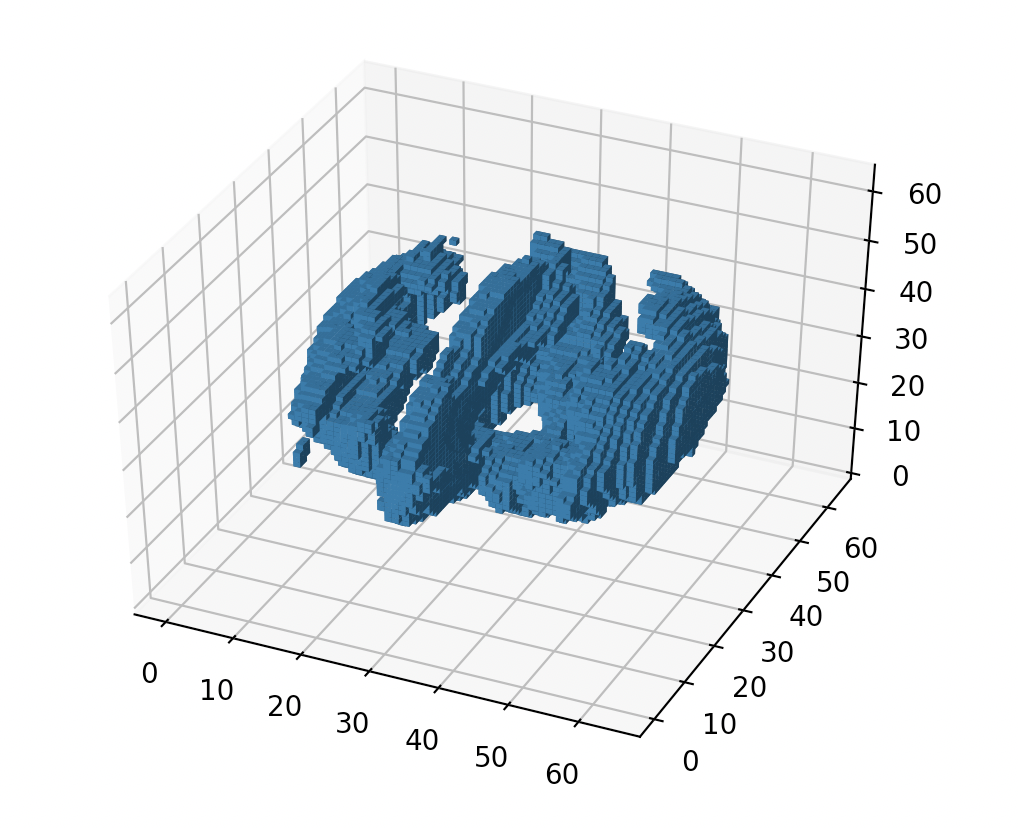
\includegraphics[scale=0.2]{custom_loss.png}
    \caption{Increased Complexity With Centroid-Weighed BCE Loss}
\end{figure}

Even with the heavily weighted center voxels and increased number of parameters,
the network was not able to learn the vascular structure. Both our VAE and GAN
networks produced similar, inaccurate results. This trend in related issues
leads us to believe that there is an inherent difficulty in training--
specifically--a Convolution Neural Network for this specific problem. The
cerebrovascular structure of the brain is an incredibly complex object to
reconstruct, evidently more so than simple, inanimate objects that
state-of-the-art CNNs are able to reconstruct. We can conclude because CNNs 
intrinsically try to find patterns within features that share parameters, this
type of network will not be able to learn the complexities of the vascular
structure. In other words, the cerebrovascular structure consists of seemingly 
random lines in space that a CNN is inherently not capable of learning because 
of its reliance on the aforementioned structure of the problem. Therefore, a 
CNN is not suitable for this reconstruction.


A possible solution to reducing the complexity of the model is to potentially slice the volumetric space into pieces. In some cases, this may help eliminate the data sparsity problem by making it easier for the model to predict an empty space within the structure. Christopher Choy et al. used a similar approach in their 3D-R2N2 model for 3D Image Reconstruction. Their novel architecture for a 3D Convolutional LSTM had LSTM blocks corresponding to different areas within the volumetric space. In essence, these separate blocks either retained or disposed of information only pertinent to that region of the 3D image as the model was fed more angles of the object. In our application, however, there is no need for LSTM blocks as each biplane view of the brain structure is consistent for every ground truth model. Despite this, the concept of splicing can still be relevant.

Given these difficulties with CNNs, a potentially better solution using deep
learning would be to create a morphology file directly from the biplane views
of the brain. In this sense, our network would act as a "middleman" between
the 2D images and the 3D model. There already exists architecture to convert 
these morphology files into 3D models, so this one extra step of converting
the images into usable files for later reconstruction may be necessary given
the constraints of our problem. Moving away from deep learning, another possible
model would a voxel-by-voxel predictor network similar to the model proposed by 
Wu, Wang \cite{ML approach}.


\section{Conclusion}
3D neurovascular reconstruction from X-ray angiography images is not feasible with the aforementioned deep learning models. The vessel structure in the brain is too complex for the 3D Autoencoder, 3D VAE, and 3D GAN. Each model outputs an inaccurate representation of the structure and should not be used for any practical purposes. However, although this deep learning approach falls short of expectations, there are other machine learning \cite{ML approach}  and probabilistic \cite{Probabililstic approach} approaches that have proven to be accurate and practical. 


\begin{thebibliography}{00}
\bibitem{Angiography Segmentation} P. Liskowski and K. Krawiec. "Segmenting Retinal Blood Vessels With Deep Neural Networks". In: \textit{IEEE Transactions on Medical Imaging} 35.11 (2016), pp.2369.
\bibitem{MVS} Po-Han Huang et al. “DeepMVS: Learning Multi-view Stereopsis”. In: CoRR abs/1804.00650 (2018). arXiv: 1804.00650. URL: http://arxiv.org/abs/ 1804.00650.
\bibitem{3DLSTM} Christopher B Choy et al. “3D-R2N2: A Unified Approach for Single and Multi-view 3D Object Reconstruction”. In: \textit{Proceedings of the European Conference on Computer Vision (ECCV)}. 2016.
\bibitem{VAE/GAN} Jiajun Wu et al. “Learning a Probabilistic Latent Space of Object Shapes via 3D Generative-Adversarial Modeling”. In: \textit{CoRR} abs/1610.07584 (2016). arXiv: 1610.07584. URL: http://arxiv.org/abs/ 1610.07584.
\bibitem{ML approach} L. Wu, Q. Wang. "Reconstruct 3D brain vasculature from multiple 2D images". (2018).
\bibitem{Probabililstic approach} M. Rempfler et al. "Reconstructin cerebrovascular networks under local physiological constraints by integer programming". In: \textit{Med Image Anal} 25.1 (Oct. 2015), pp. 86-94.
\end{thebibliography}
\vspace{12pt}

\end{document}
